%& C:\Users\RANGAR~1\AppData\Roaming\TikzEdt\TikzEdt\023~1.0\TEMP_H~1
\begin{document}
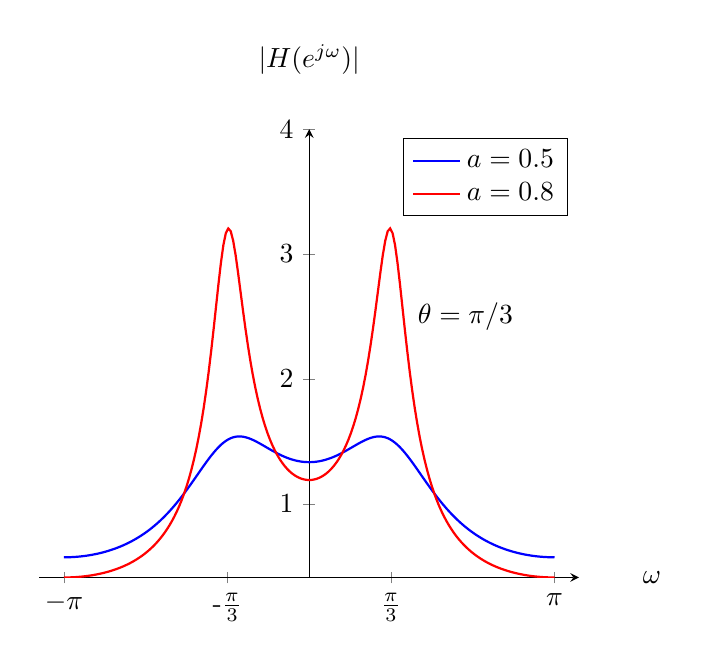
\begin{tikzpicture}
	
	\begin{axis}[
		xlabel=$\omega$,
		ylabel=$|H(e^{j\omega})|$,
		axis lines = middle,
		xmin = -1.1*pi,
		xmax = 1.1*pi,
		ymax = 4,
    	xtick={-3.14159, -1.0472, 1.0472,  3.14159},
    	xticklabels={$-\pi$, -$\frac{\pi}{3}$,  $\frac{\pi}{3}$,  $\pi$},
    	y label style={at={(axis description cs:0.5,1.1)},anchor=south},
    	x label style={at={(axis description cs:1.1,0)},anchor=west},    	
	]
	\def\r{0.5}
	\def\ct{0.5}%cos(theta)
	\addplot[blue, thick, domain=-pi:pi, samples=201] {1/sqrt(1 + 4*\r^2*\ct^2 + \r^4 - 4*\r*\ct*cos(deg(x)) + 2*\r^2*cos(2*deg(x)) -4*\r^3*\ct*cos(deg(x))*cos(2*deg(x)) -4*\r^3*\ct*sin(deg(x))*sin(2*deg(x)) )};
	\def\r{0.8}
	\addplot[red, thick, domain=-pi:pi, samples=201] {1/sqrt(1 + 4*\r^2*\ct^2 + \r^4 - 4*\r*\ct*cos(deg(x)) + 2*\r^2*cos(2*deg(x)) -4*\r^3*\ct*cos(deg(x))*cos(2*deg(x)) -4*\r^3*\ct*sin(deg(x))*sin(2*deg(x)) )};
	\legend{$a=0.5$, $a=0.8$}
	\node at (axis cs:2, 2.5) {$\theta = \pi/3$};
	\end{axis}

\usetikzlibrary{calc}
\pgftransformreset
\node[inner sep=0pt,outer sep=0pt,minimum size=0pt,line width=0pt,text width=0pt,text height=0pt] at (current bounding box) {};
%add border to avoid cropping by pdflibnet
\foreach \border in {0.1}
  \useasboundingbox (current bounding box.south west)+(-\border,-\border) rectangle (current bounding box.north east)+(\border,\border);
\newwrite\metadatafile
\immediate\openout\metadatafile=\jobname_BB.txt
\path
  let
    \p1=(current bounding box.south west),
    \p2=(current bounding box.north east)
  in
  node[inner sep=0pt,outer sep=0pt,minimum size=0pt,line width=0pt,text width=0pt,text height=0pt,draw=white] at (current bounding box) {
\immediate\write\metadatafile{\p1,\p2}
};
\immediate\closeout\metadatafile
\end{tikzpicture}

\end{document}
d{tikzpicture}

\end{document}
ment}
cument}

